\chapter{物理节点单故障可生存性虚拟网络嵌入算法}
\section{问题描述}
在这一部分中,我们首先介绍了虚拟网络嵌入的基本概念,然后提出了我们的可生存虚拟网络嵌入问题。
\subsection{虚拟网络嵌入}
我们将\textbf{虚拟网络}VN表示为无向图$G (V,E)$,其中$V$和$E$分别是虚拟节点和虚拟链路的集合。每个虚拟链路$e_{ij}$具有带宽需求$d_{ij}$。每个虚拟节点$v_i$ 具有计算容量需求$d_i$。对于虚拟节点$v_i$,需要在虚拟节点上执行的虚拟函数表示为$f(i)$。如图\ref{fig:VirtualNetworkRequest}所示虚拟网络$G (V,E)$ 具有虚拟节点集$V=\{v_1,v_2,v_3,v_4\}$和虚拟边集$E= \{e_{12},e_{13},e_{14},e_{23}\}$。需要在这些虚拟节点上执行的虚拟函数是$f(1)=f_1$, $f(2)=f_2$, $f(3)=f_3$, $f(4)=f_4$。

\begin{figure*}
\centering
% Requires \usepackage{graphicx}
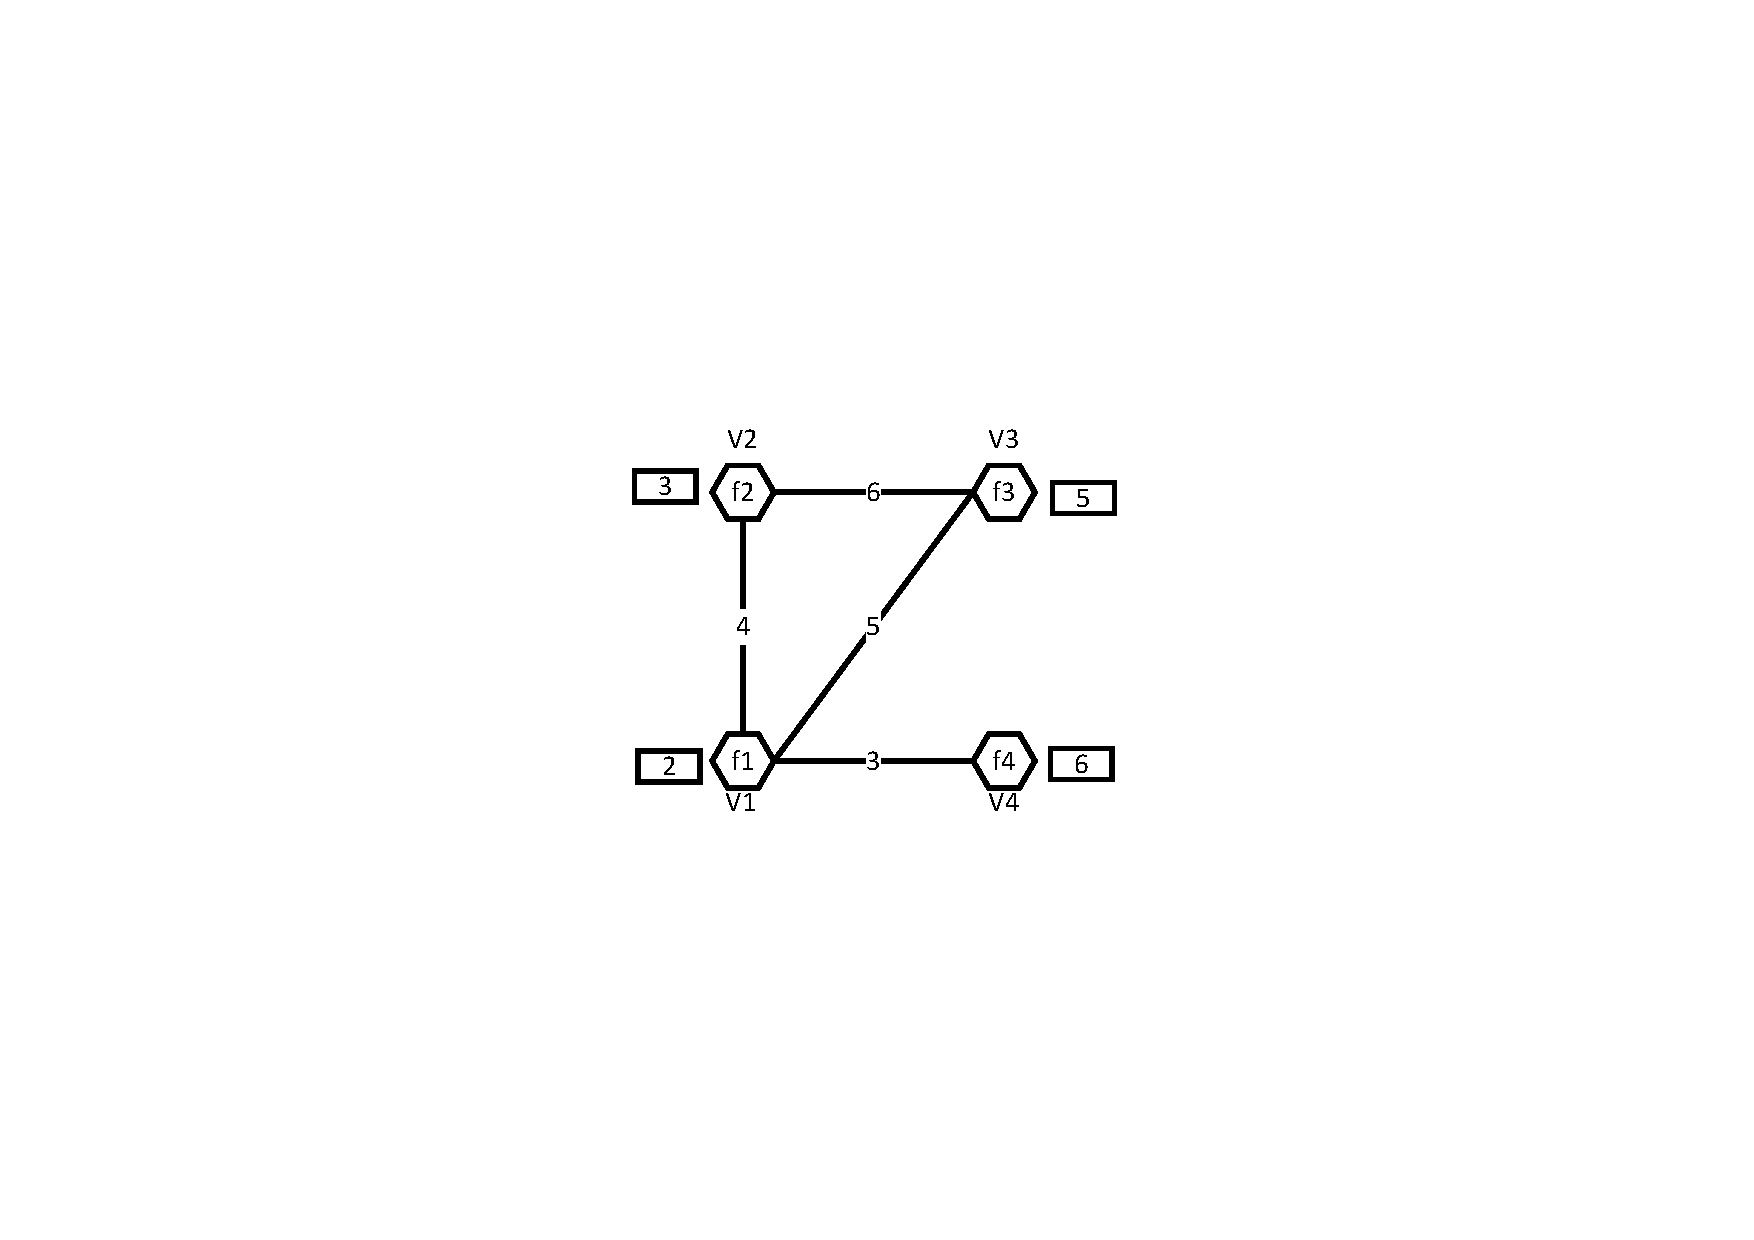
\includegraphics[width=4in]{figures/VirtualNetworkRequest}\\
\caption{虚拟网络请求$G(V,E)$, $V=\{v_1,v_2,v_3,v_4\}$, $E=\{e_{12},e_{23},e_{13},e_{14}\}$,  $f(i)=\{f_1,f_2,f_3,f_4\}$, $d_i=\{2,3,5,6\}$, $d_{ij}=\{4,5,3,6\}. $
}\label{fig:VirtualNetworkRequest}
\end{figure*}

我们将底层\textbf{物理网络}建模为一个无向图$G (S,L)$,其中$S$和$L$ 分别是物理节点和物理链路的集合。对于物理节点$s_i$,我们使用$F(i)$ 和$c_i$分别表示可以在该节点上执行的一组可行的虚拟功能和可用的计算能力。每个物理链路$l_{ij}$ 都有可用带宽$b_{ij}$。如图\ref{fig:PhysicalNetwork}所示的物理网络$G (S,L)$,物理节点集合$S=\{s_1,s_2,s_3,s_4,s_5,s_6,s_7,s_8\}$,链路集合$L=\{l_{12},l_{13},l_{14},l_{15},l_{23},l_{25},l_{35},l_{36},l_{37},l_{47},l_{58}\}$,
每一个物理节点的可行的虚拟功能$F(1)=\{f_1\}$, $F(2)=\{f_2,f_3\}$, $F(3)=\{f_3\}$, $F(4)=\{f_4\}$, $F(5)=\{f_1,f_2\}$, $F(6)=\{f_1,f_4\}$, $F(7)=\{f_2,f_3\}$,$F(8)=\{f_2\}$。

\begin{figure*}
\centering
% Requires \usepackage{graphicx}
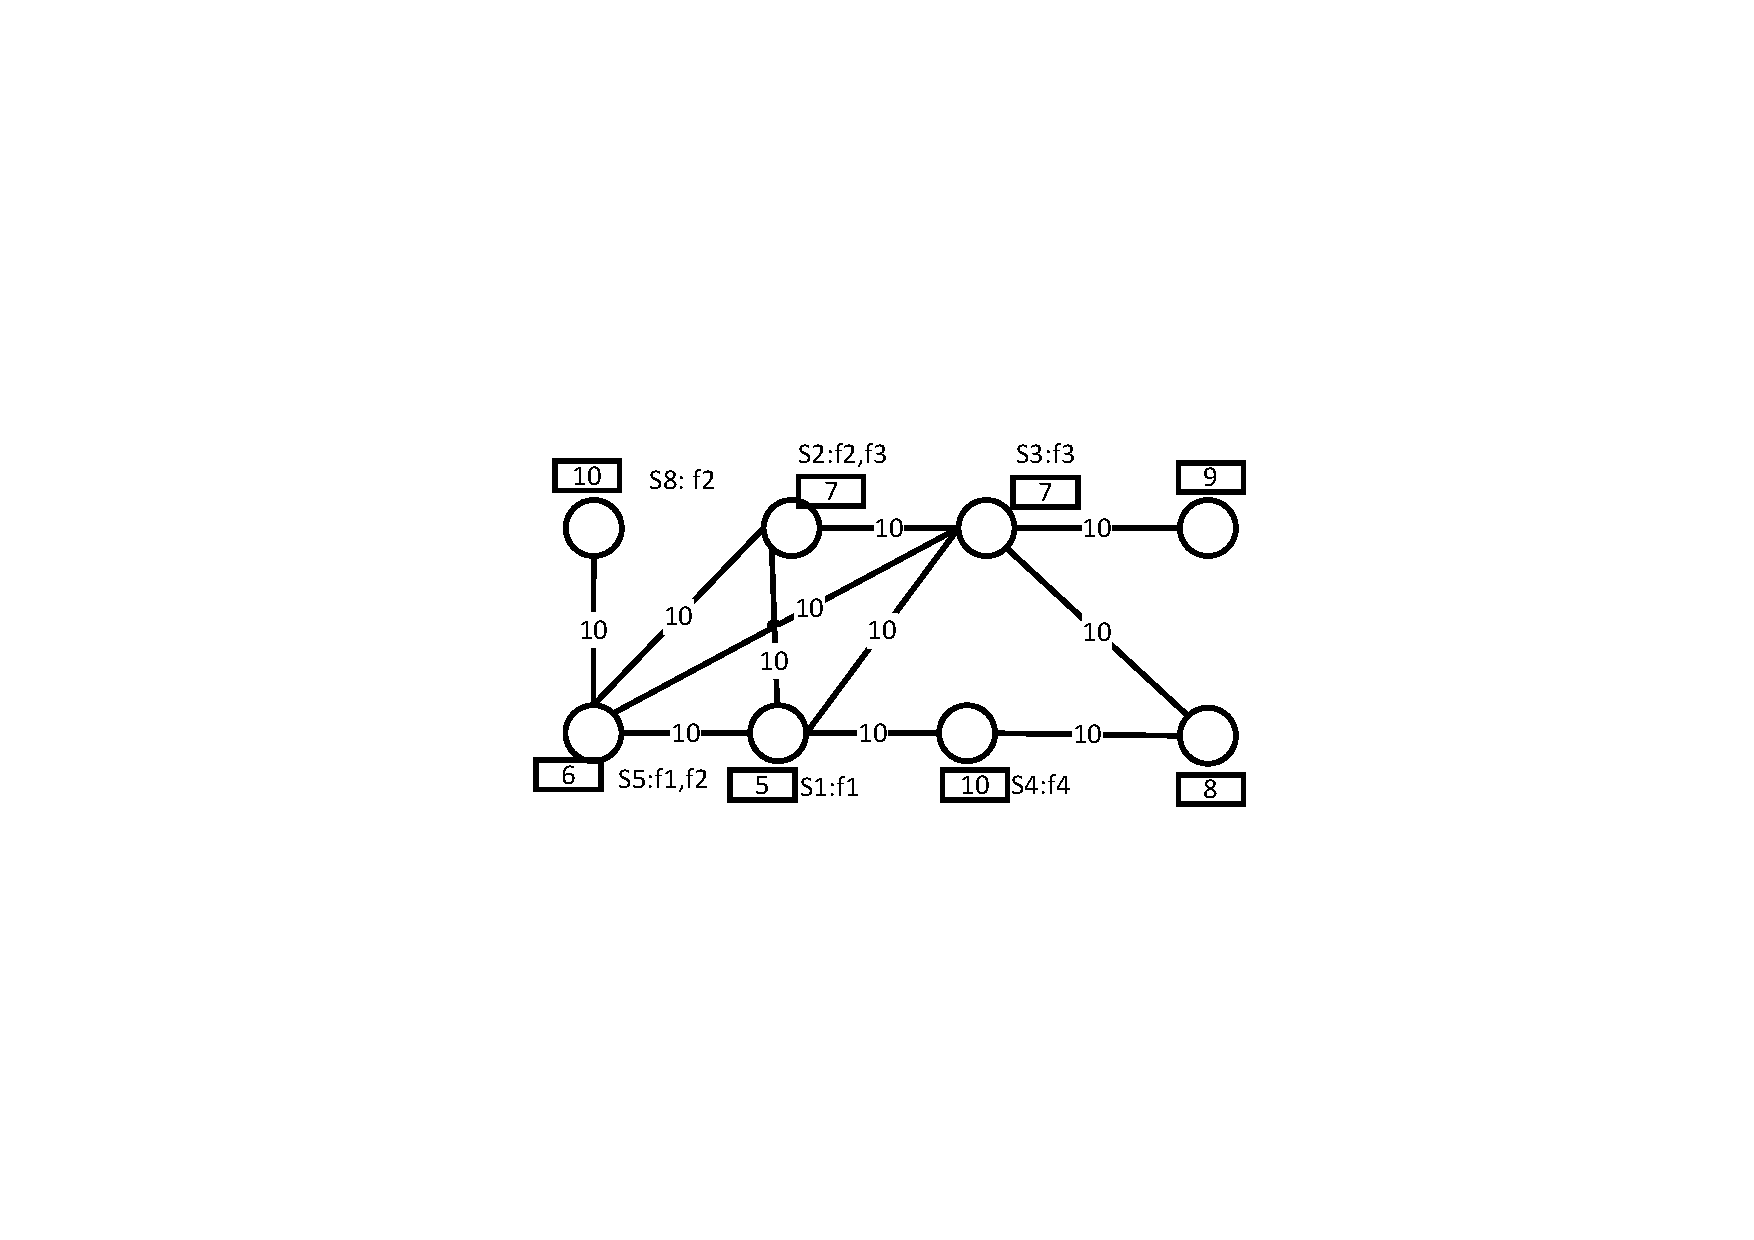
\includegraphics[width=4in]{figures/PhysicalNetwork}\\
\caption{底层物理网络$G(S,L), S=\{s_1,s_2,s_3,s_4,s_5,s_6,s_7,s_8\}, L=\{l_{12},l_{13},l_{14},l_{15},l_{23},l_{25},l_{35},l_{36},l_{37},l_{47},l_{58}\}, F(i)=\{\{f_1\},\{f_2,f_3\},\{f_3\},\{f_4\},\{f_1,f_2\},\{f_1,f_4\},\{f_2,f_3\},\{f_2\}\}, c_i=\{5,7,7,10,6,9,8,10\}, b_{ij}=\{10,10,10,10,10,10,10,10,10,10,10\}$}\label{fig:PhysicalNetwork}
\end{figure*}

在给定VN请求$G (V,E)$的情况下,虚拟网络嵌入问题的目的是将该请求映射到物理网络$G (S,L)$ 上,同时提供所需的足够资源。一个可行的嵌入应该满足节点容量约束、链路带宽约束和功能类型约束这三个约束条件。

对于一个虚拟节点$v_i$,物理节点$s_j$只在节点容量约束和功能类型两种情况满足约束条件(即${f_i} \in {F_j}$)下被映射这个虚拟节点。即节点的容量请求应满足$d_i\leq c_j$的物理节点,虚拟节点上需要执行的虚拟功能属于物理节点$s_j$上可以执行的虚拟功能${f_i} \in {F_j}$。 如果物理节点$s_j$ 满足这两个约束,则节点映射是可行的,并且我们表示这样的映射为$\phi ({v_i}) = {s_j}$。

对于在两个已经映射到两个物理节点$s_{i'}$和$s_{j'}$(即$\phi({v_i}) = {s_{i'}}$ 和$\phi({v_j}) = {s_{j'}}$) 的虚拟节点之间的虚拟链路$e_{ij}$,在链路带宽约束下$d_{ij}\leq b_{i'j'}$(其中$b_{i'j'}$是连接物理节点$s_{i'}$ 和$s_{j'}$的可用带宽),这条虚拟链路$e_{ij}$可以映射到物理路径$p_{\phi({v_i}) \phi({v_j})}$,则表示可行的链路映射为$\rho(e_{ij}) = p_{\phi({v_i}) \phi({v_j})}$。

显然,为了找到一个可行的虚拟网络嵌入,我们需要找到两个映射函数$\phi$ 和$\rho$来将所有虚拟节点映射到物理节点,以及将所有链路链接映射到物理路径。

如图\ref{fig:VirtualNetworkEmbedding}所示一个可行的虚拟网络嵌入,将图\cite{fig:VirtualNetworkRequest}中的虚拟网络嵌入到图\cite{fig:PhysicalNetwork}中的物理网络中,其中虚拟节点$v_1$嵌入到物理节点$s_1$,虚拟节点$v_2$嵌入到物理节点$s_2$,虚拟节点$v_3$嵌入到物理节点$s_3$,虚拟节点$v_4$嵌入到物理节点$s_4$。在图\ cite{fig:PhysicalNetwork} 中,我们还展示了在这样的映射之后物理网络中已经占用的和可用的资源。例如,对于物理节点$s_1$,其占用的计算容量为2,可用容量为5。

给定VN请求$G(V,E)$和物理网络$G(S,L)$,对于可行映射,我们将映射的物理图表示为$G\left( {\hat S,P} \right)$,其中$\hat S$是容纳虚拟节点的物理节点集,其中$\hat S = \{ {s_{i'}}:\phi({v_i}) = {s_{i'}},for\ \ {\rm{ }}all\ {v_i} \in V,{s_{i'}} \in S\}$ 和$P$ 是路径集,其中每个路径都持有一个虚拟链路$P = \{ p_{\phi({v_i}) \phi({v_j})}:\rho(e_{ij}) = p_{\phi({v_i}) \phi({v_j})}{\rm{ }}, for\ all,{e_{ij}} \in E\}$。由于每个虚拟链路对应一个物理网络路径,该路径由多个物理链路组成,因此我们还将$G\left( {\hat S,\hat L} \right)$表示为占领的物理网络$\hat L = \{ {l_{pg}}:{l_{pg}} \in {p_{s_{i'}s_{j'}}}, \rho(e_{ij}) = p_{\phi({v_i}) \phi({v_j})},for\ all\ {e_{ij}} \in E,{l_{pg}} \in L\}$。

已经有了许多研究虚拟网络嵌入问题\cite{fischer2013virtual};,因为本文的重点不是虚拟网络嵌入算法,我们采用了\cite{lischka2009virtual} 中的算法作为基本的虚拟网络嵌入算法。


\begin{figure*}
\centering
% Requires \usepackage{graphicx}
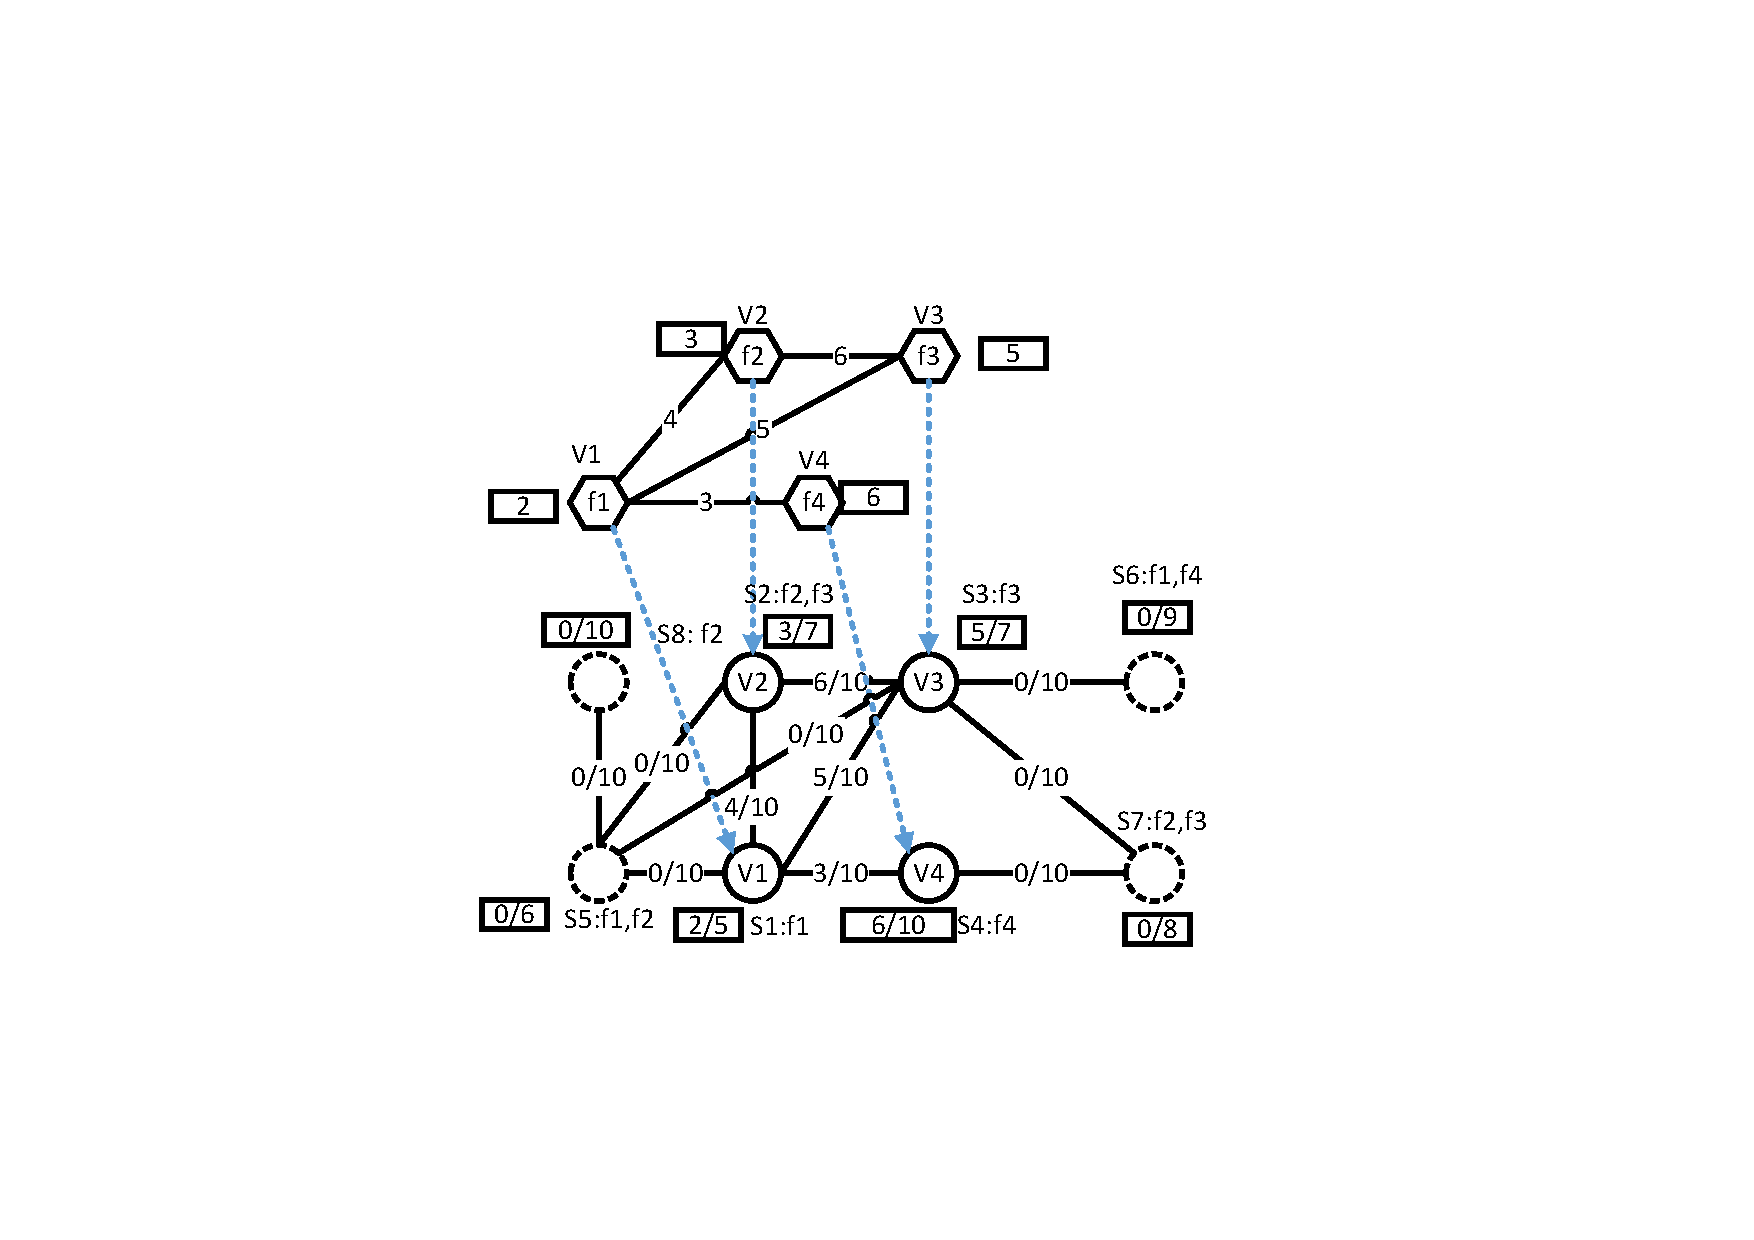
\includegraphics[width=4in]{figures/VirtualNetworkEmbedding}\\
\caption{节点映射$v_1\rightarrow s_1, v_2\rightarrow s_2, v_3\rightarrow s_3, v_4\rightarrow s_4$,链路映射$e_{12}\rightarrow l_{12},e_{23}\rightarrow l_{23},e_{13}\rightarrow l_{13},e_{14}\rightarrow l_{14}$.}\label{fig:VirtualNetworkEmbedding}
\end{figure*}
\subsection{可生存性虚拟网络嵌入}
由于恶意攻击、自然灾害、无意中断电缆、计划维护、设备故障、物理节点承载的虚拟节点可能会遭受不可避免的故障。当单个或多个物理网络组件发生故障时,VN 中可能会发生故障,从而造成财务损失。一般来说,多个物理节点的同时失效是相互独立的,单个节点的失效通常发生在大多数时间\cite{yeow2010designing}。本文研究了单节点失效的可生存虚拟网络嵌入问题。在本章中,我们将讨论如何将我们的算法扩展到多节点故障的场景中。

对于VN请求$G (V,E)$和物理网络$G (S,L)$,给出了其占用物理网络的可行映射,在任何一个物理节点发生故障时,增加最小备份物理资源以提供可生存性的网络服务。

节点故障不仅影响运行在失效的物理节点上的可视化服务,而且会终止通过该节点的所有通信。物理节点 $ {s_i} \in S $的失效导致相邻物理链路的失效${L_i} = \left\{ {{l_{ik}}:k \in N(i)} \right\}$,其中${N(i)}$ 是节点$ {s_i} $的邻居节点。

由于我们无法预测哪个节点将失效,即使我们知道多个节点不会同时失效,为了处理单节点故障,一个直接的方式是为VN请求中的每个虚拟节点提供专用备份资源,也称为1+1 保护方案。如图\cite{fig:One2OneProtection}所示利用一个例子来说明这种直截了当的方法。在该示例中,将具有4个虚拟节点的虚拟网络映射到物理网络,其中4 个物理节点参与了这样的嵌入。为了提供1 +1 保护方案,在图中添加了4个备份节点、8 个备份链路。

1+1保护方案虽然实现简单,但需要大量的备份资源.我算法的目的是以最小的备份资源成本提供可生存的网络服务。

\begin{figure}
\centering
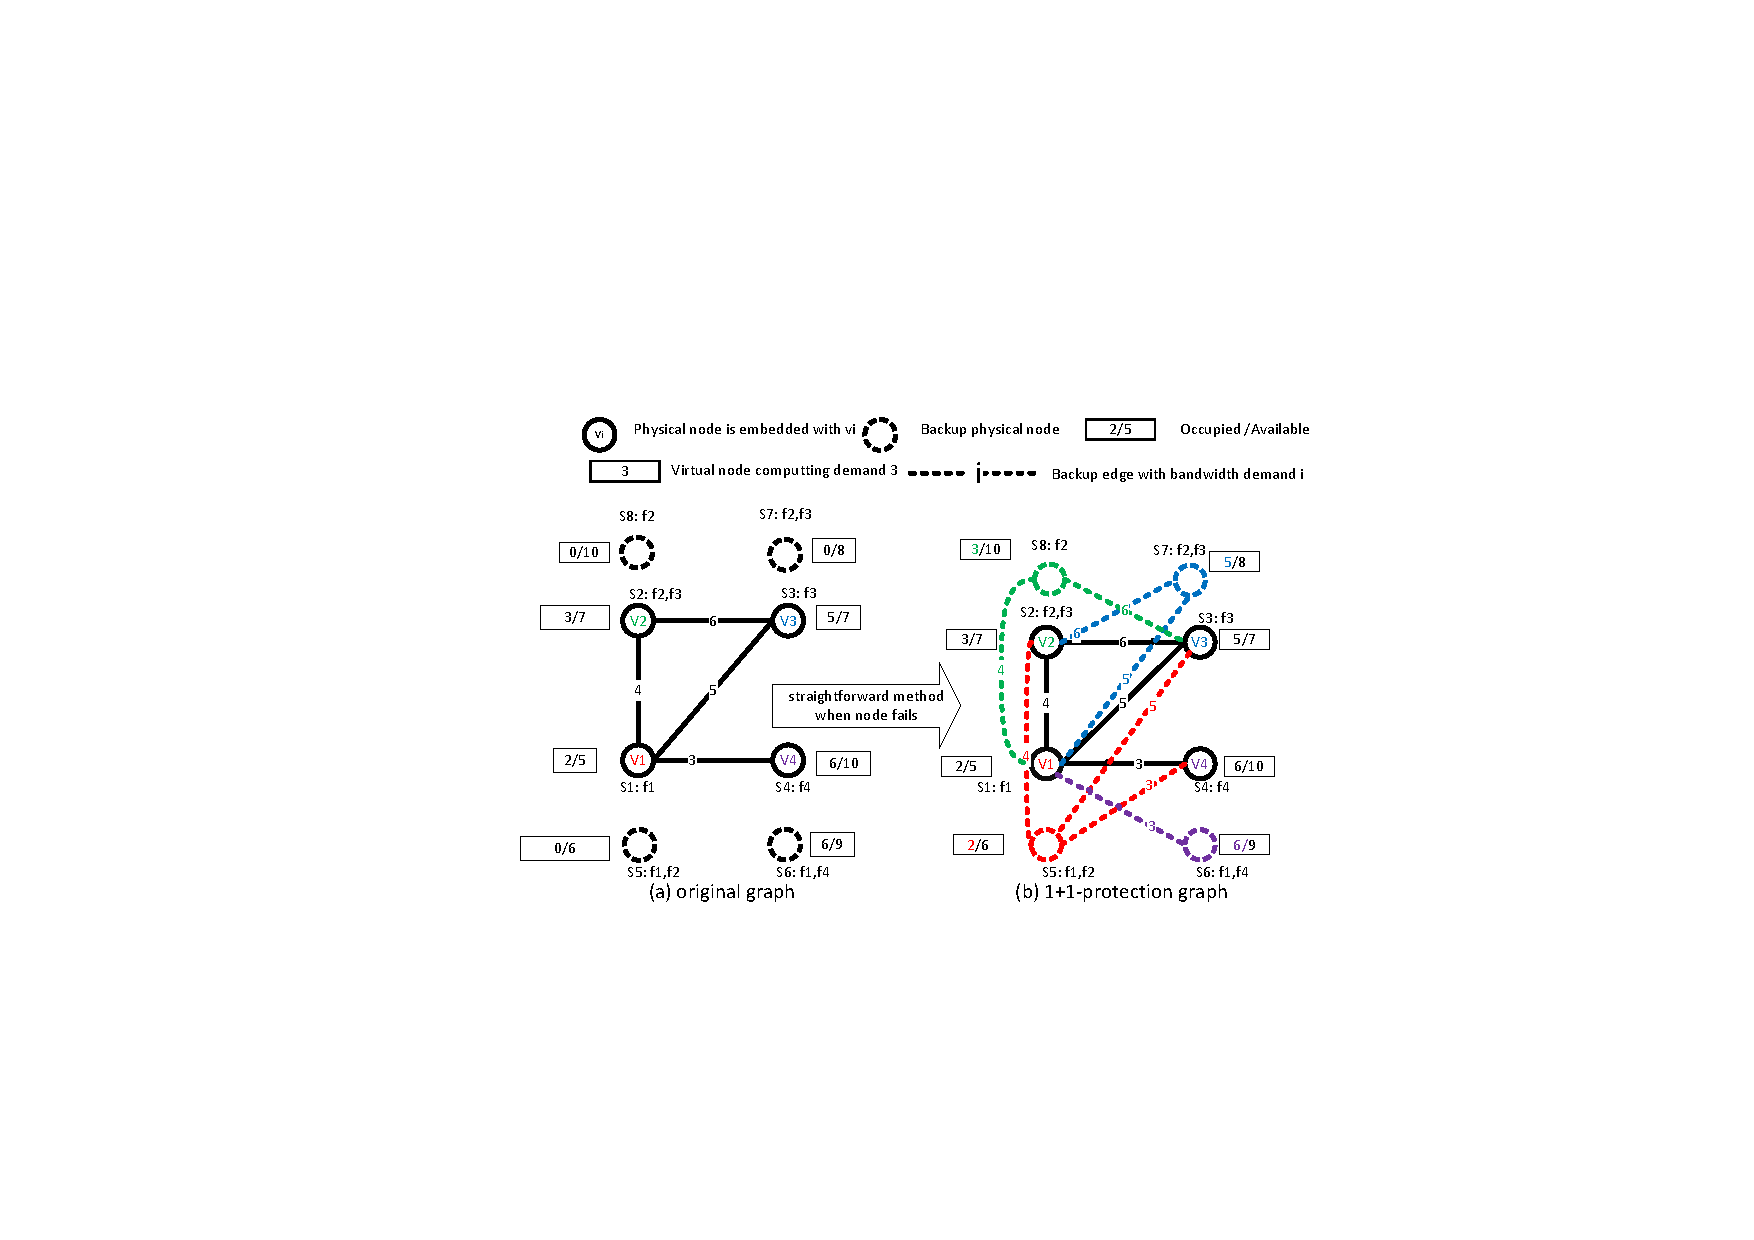
\includegraphics[width=3.5in]{figures/One2OneProtection}\\
\caption{1+1-保护机制}\label{fig:One2OneProtection}
\end{figure}
\section{基于问题公式的图分解}
可生存虚拟网络嵌入需要添加备份资源,以保证当任何一个物理节点失效时,剩余的物理资源加上备份资源仍然可以支持失效的嵌入。为了便于在节点失效时找到可行的嵌入,本节首先对虚拟网络进行分解,物理网络以星型为基础的局部组件。在此基础上,提出了一种新的二分图,并将具有最小备份资源的可生存虚拟网络嵌入问题转化为一个基于定义良好的二分图的虚拟星图分配问题。
\subsection{星型图分解}
将虚拟网络分解为虚拟局部星型图。每个虚拟局部星型图与一个虚拟节点相关联。给出虚拟节点$v_i$,相应的虚拟本地星型图被定义为属性化单层根树,并表示为

\begin{equation}
VirtualStar(v_i)=(v_i, \phi(v_i), d_i, f_i, D_i, N_i)
\label{eq:virtualstar}
\end{equation}


其中,$N_i$是虚拟网络中的相邻节点集,并与节点$v_i$相关联的带宽需求集${D_i} = \left\{ {{d_{ij}}|{v_j} \in {N_i}} \right\} $。注意,VirtualStar($v_i$)包括节点映射信息$\phi(v_i)$。因为我们希望最小化备份资源以提供可生存的网络服务,在节点失效前重复使用映射可能减少额外资源,使系统保持稳定的一个很好的选择。在虚拟星型图结构中,根节点和它的邻居节点存在链路,但是根节点的邻居节点之间不存在链路。

物理网络被分解为物理局部星型图。同样,每个物理局部星型图与一个物理节点相关联。给定物理节点$s_j$,对应的物理局部星型图被定义为属性化单层根树,并表示为
\begin{equation}
PhysicalStar(s_j)=(s_j, \phi^{-1}( s_j), c_j, F(j), \phi(N(\phi^{-1}( s_j))), a)
\label{eq:physicalstar}
\end{equation}

其中$\phi^{-1}( s_j)$是映射到物理节点$s_j$的虚拟节点集,$N(\phi^{-1}( s_j))$ 是$\phi^{-1}( s_j)$中虚拟节点的相邻节点,$\phi(N(\phi^{-1}( s_j)))$ 是承载这些邻居的物理节点,$c_j$是节点容量,$F(j)$ 是$s_j$支持的虚拟功能,$a$是一个1 位的单比特,它的值为0 或1,以指示这个物理节点是否开启和设置了虚拟机。与虚拟星型图类似,在物理星型图结构中,根节点与相邻节点之间存在边,相邻节点之间不存在边。定义在\ref{eq:virtualstar} 和\ref{eq:physicalstar} 中的虚拟星型图和物理星型图很好地捕获了隐藏在VN 请求中的局部结构,以保持节点与其相邻节点之间的关系。基于虚拟局部星型图和物理虚拟星型图,虚拟网络和物理网络可以分解为多个组件。

\subsection{二分图}
构造了一个二分图$G=\{V_1,V_2,E\}$来表示虚拟网络与物理网络之间的关系。$V_1$ 和$V_2$分别表示虚拟星型图和物理星型图的集合。如果VirtualStar($v_i$) 的虚拟功能 $f_i$能在具有${f_i} \in {F_j}$的物理节点$s_j$上执行,则在边集$E$中添加边缘$e(i,j)$,以连接VirtualStar($v_i$) 和PhysicalStar($s_j$)。

我们的目标是最小化备份资源以提供可生存性的服务。为了服务于目标,给定边$e(i,j)$,我们定义了边权$w(i,j)$作为备份资源成本。当节点发生故障时,将虚拟星型图($v_i$) 映射到物理星型图($s_j$)。根据虚拟节点$v_i$映射到物理节点$s_j$ 节点是否失败,在两种不同的情况下定义了边权重$w(i,j)$。
\begin{equation}
w(i,j) = \left\{ {\begin{array}{*{20}{c}}
   { \alpha \sum\limits_{\phi ({v_k}) \notin \phi (N({\phi ^{ - 1}}({s_j})))} {{d_{ik}}} } & {{v_i} \in {\phi ^{ - 1}}({s_j}),v_k \in N(i)}  \\
   {\alpha \sum\limits_{k \in N(i)} {{d_{ik}}}  + \beta {M_m} + \lambda {c_i} + \theta } & {{v_i} \notin {\phi ^{ - 1}}({s_j}),v_k \in N(i)}  \\
\end{array}} \right.
\label{eq:edge weight}
\end{equation}
在公式.(\ref{eq:edge weight})中,$\theta$ 被定义如下.
\begin{equation}
\theta  = \left\{ {\begin{array}{*{20}{c}}
   {{C_s}} & {a = 0}  \\
   0 & {a = 1}  \\
\end{array}} \right.
\end{equation}

在第一种情况下(${v_i} \in {\phi ^{ - 1}}({s_j})$),由于虚拟节点$v_i$ 映射到的物理节点$s_j$失效,节点容量需求已经得到满足,因此当将虚拟星($v_i$) 映射到物理星型图($s_j$) 时只需要带宽备份成本。对于每个相邻的$v_k \in N(i)$,如果物理节点${\phi ({v_k}) \notin \phi (N({\phi ^{ - 1}}({s_j})))}$包含失效虚拟节点$v_k$,则应添加具有带宽$d_{ik}$的新路径作为备份资源。因此,在这种情况下,备份成本只包括带宽成本,并表示为$ { \alpha \sum\limits_{\phi ({v_k}) \notin \phi (N({\phi ^{ - 1}}({s_j})))} {{d_{ik}}} }$,其中$\alpha$是单位带宽成本。

在第二种情况下(${v_i} \notin {\phi ^{ - 1}}({s_j})$),由于虚拟节点$v_i$ 在节点失效之前没有映射到物理节点$s_j$,因此需要将虚拟节点$v_i$ 迁移到物理节点$s_j$。 因此,边权重$w(i,j)$)包括节点容量成本、路径带宽成本和迁移成本,以便在物理节点失效时将虚拟节点从物理节点迁移到另一个物理节点。此外,如果备份物理节点$s_j$之前不包含任何虚拟节点,则将虚拟节点迁移到该物理节点也会引入虚拟机启动成本,其表示为$C_s$。

如图\ref{fig:StarRepresentation}所示显示了当物理节点$s_1$失效时这种二分图的一个例子。这种二部图的边权可以用矩阵\ref{lab:Node1FaliureAlignmentMatrixNew} 表示。
\begin{figure}
\centering
% Requires \usepackage{graphicx}
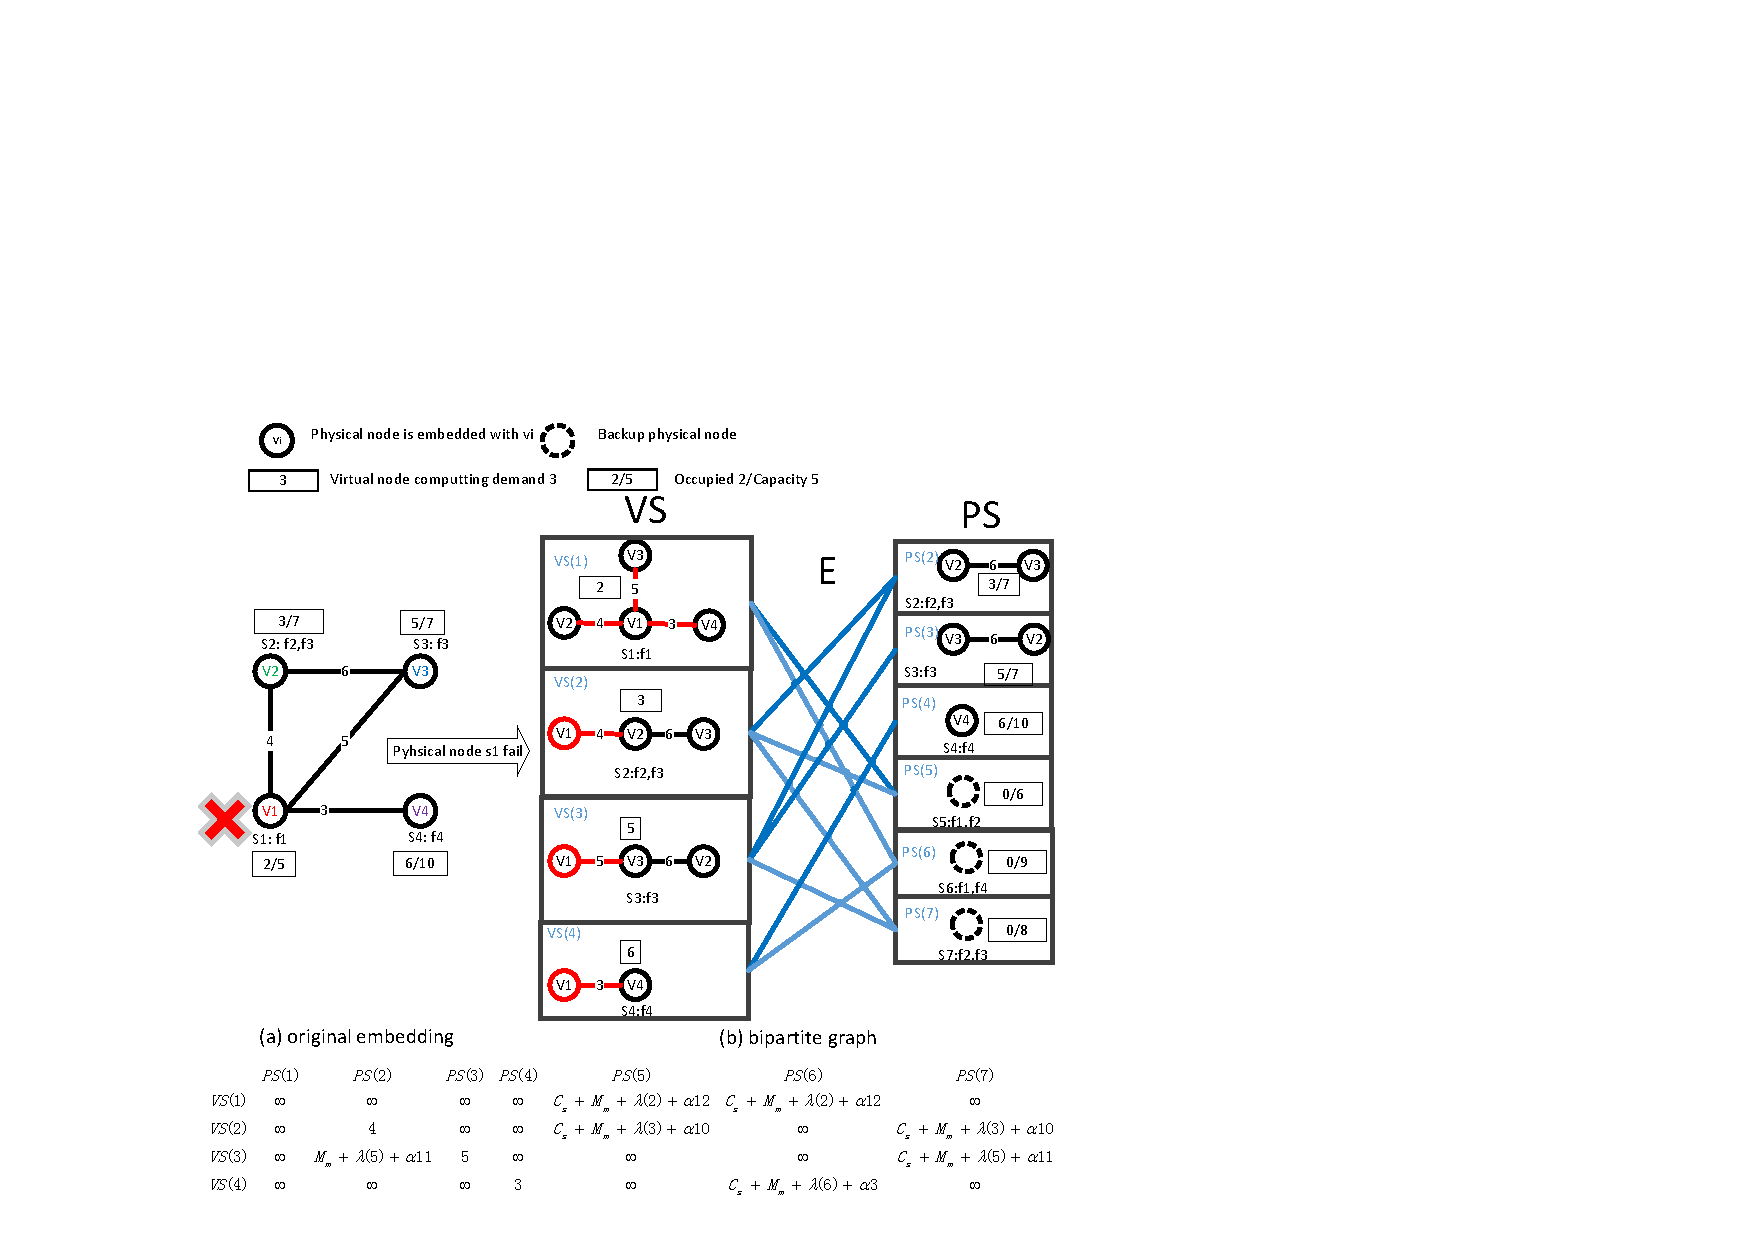
\includegraphics[width=4in]{figures/StarRepresentation}\\
  \caption{VirtualStar($v_i$)的组件,和当物理节点$s_1$失效时的PhysicalStar($s_j$)}\label{fig:StarRepresentation}
\end{figure}

\begin{equation*}
\small{
 {\begin{array}{*{20}{c}}
&R_{S_{1}}&R_{S_{2}}&R_{S_3}&R_{S_4}&R_{S_5}&R_{S_6}&R_{S_{7}}\\
{L_{V_1}}&\infty&\infty&\infty&\infty&\fbox{$C_{s}+M_{m}$+(2)+12}&C_{s}+M_{m}+(2)+12&\infty\\
L_{V_2}&\infty&\fbox{4}&\infty&\infty&C_{s}+M_{m}+(3)+10&\infty&C_{s}+M_{m}+(3)+10\\
L_{V_3}&\infty&M_{m}+(5)+11&\fbox{5}&\infty&\infty&\infty&C_{s}+M_{m}+(5)+11\\
L_{V_4}&\infty&\infty&\infty&\fbox{3}&\infty&C_{s}+M_{m}+(6)+3&\infty\\
\end{array}}
}
\label{lab:Node1FaliureAlignmentMatrixNew}
\end{equation*}


对于虚拟节点$v_i$,如果它的虚拟功能不能在具有$f(i) \notin F(i)$的物理节点$s_j$中执行,则没有边连接$VirtualStar(v_i)$ in $V_1$和$PhysicalStar(s_j)$ in $V_2$。为了便于问题表述,我们将边权设为$\infty $。例如,由于$v_1$的虚拟功能是$f_1$,所以它不能在物理节点$s_2$中执行。因此,与$VirtualStar(v_1)$和$PhysicalStar(s_2)$ in $V_2$连接时,不添加任何边,我们设置$w(1,2)=\infty$。

对于$VirtualStar(v_2)$,因为$v_2$最初由$s_2$持有,但是,当物理节点$s_1$(最初持有$v_1$)失效时,虚拟链路$e_{12}$无法映射到物理网络。我们应该找到一条连接$\phi(v_2)$和$\phi(v_1)$满足带宽需求$d_{12}=4$的新路径。因此,边权系数$VirtualStar(v_2)$和$PhysicalStar(s_2)$的值为4。

当节点$s_1$失效时,它直接影响虚拟节点$v_1$。 由于$s_5$可以执行虚拟功能$f_1$,我们可以添加一个边来连接$VirtualStar(v_1)$和$PhysicalStar(s_5)$。 然而,在由于$s_5$以前没有设置虚拟机,因此还引入了虚拟机的启动成本$C_s$。 因此,链路权重为$C_s$(启动成本)+$M_m$(迁移成本)+3(节点容量成本)+10(带宽成本)。

\subsection{问题定义}
为了提供可生存的服务,每个虚拟星型图(根虚拟节点和连接根节点及其相邻节点的虚拟链路)都应该映射到物理星型图。假设虚拟网络由n个虚拟节点组成,因此n个虚拟星型图。物理网络由m 个物理节点组成,从而构成m 个物理星型图。在等式\ref{eq:indication}中,我们使用二进制位$M_{ij}$ 来表示第i个虚拟星型图是否映射到第j物理星型图。

\begin{equation}
{M_{ij}} = \left\{ {\begin{array}{*{20}{c}}
   1 & {map \ v_i \  to  \ s_j}  \\
   0 & {otherwise}  \\
\end{array}} \right.
\label{eq:indication}
\end{equation}

当物理节点发生故障时,为了使备份资源成本最小化,可生存性虚拟网络嵌入问题可以定义如下:
\begin{equation}
\begin{array}{*{20}{c}}
   {\mathop {\min }\limits_{{M_{ij}}} } & {\sum\limits_{i = 1}^n {\sum\limits_{j = 1}^m {{M_{ij}}{w_{ij}}} } }  \\
   {s.t.,} & {\sum\limits_{i = 1}^n {{d_i}{M_{ij}}}  \le {c_j}}  \\
   {} & {\sum\limits_{j = 1}^m {{M_{ij}}}  \le 1}  \\
   {} & {{M_{ij}} = \{ 0,1\} }  \\
\end{array}
\label{eq:problem formulation}
\end{equation}

其中${\sum\limits_{i = 1}^n {\sum\limits_{j = 1}^m {{M_{ij}}{w_{ij}}} } }$ 表示当物理节点失效时将所有虚拟星型图映射到物理星型图的总备份资源成本。在公式\ref{eq:problem formulation} 中,${\sum\limits_{i = 1}^n {{d_i}{M_{ij}}}  \le {c_j}}$是物理节点的容量约束,也就是说,即使允许将多个虚拟节点映射到一个物理节点,总容量需求不应大于物理节点的容量。${\sum\limits_{j = 1}^m {{M_{ij}}}  \le 1}$ 表示一个虚拟星型图只映射到一个物理星型图。

显然,公式\ref{eq:problem formulation}中定义的问题是一个二进制ILP 问题,根据Karp 的21 个NP-完全问题\cite{karp1975computational},它是一个一般的NP-complete问题。

\textbf{Theorem 1} 定义为公式\ref{eq:problem formulation}是一个NP-complete 问题.
\begin{proof}
如果只有一个物理节点m=1,则我们的可生存虚拟网络嵌入问题可以退化为单背包问题,即NP-完全问题。在实际应用中,m通常大于1,单背包问题是可生存虚拟网络嵌入问题的子问题,给出的可行解在多项式时间内很容易验证,根据计算机复杂性领域上的可归约性定理\cite{wood1987theory},很容易得出我们在\ref{eq:problem formulation}中定义的也是NP-complete 的结论。
\end{proof}

\subsection{动态规划方法}
\label{lab:DynamicProgrammingEquation}
虽然求解ILP公式会得到最小成本的生存虚拟网络嵌入,但其指数时间复杂度使得这种方法在大型物理网络中嵌入虚拟网络是不可行的。在这一部分中,我们提出了一种基于动态规划的算法,该算法仅具有多项式时间复杂度,因此对于实际的网络系统是可行的方法。

为了描述基于动态规划的算法,我们定义了$dp[i][{x_1}][{x_2}] \ldots [{x_m}]$ 表示以最小备份资源代价将第前面$i$($0 \le i \le n $)个虚拟星型图放置到物理网络中的m个物理星型图中,其容量限制为$ x_1$, $ x_2$, $\ldots$, $x_m$。

第$i$个虚拟节点可以选择放置在任何一个存活的的物理星型图上。设$\theta (i,j)$ 表示已经将原先$i-1$个虚拟节点最佳放置后在将第$i$个虚拟节点放置到第j 个物理节点的备份资源成本。$\theta (i,j)$表示如下:
\begin{equation}
\theta (i,j) = \left\{ {\begin{array}{*{20}{c}}
{dp[i - 1][x_1][{x_2}] \ldots [{x_j} - {d_i}] \ldots [{x_m}] + {w_{ij}}}\\
\infty
\end{array}} \right.\begin{array}{*{20}{c}}
{({x_j} \ge {d_i},{f_i} \in {F_j})}\\
{otherwise}
\end{array}
\label{eq:place i to j}
\end{equation}
在等式\ref{eq:place i to j}中,如果物理节点$x_j$的容量限制大于容量需求$d_i$ 并且在物理节点${f_i} \in {F_j}$能执行虚拟功能$f_i$,则 $\theta (i,j)$ 是已经放置前面i−1个最佳虚拟星型图的代价和(即$dp[i-1][{x_1} - {d_i}][{x_2}] \ldots [{x_m}]$)和将虚星($v_i$) 映射到物理星($s_1$)的成本(即$w_{i1}$)。

基于$\theta (i,j)$,$dp[i][{x_1}][{x_2}] \ldots [{x_m}]$可通过以下动态规划函数计算。
\begin{equation}
dp[i][{x_1}][{x_2}] \ldots [{x_m}] = min\{\theta (i,1),\theta (i,2),\ldots,\theta (i,j),\ldots,\theta (i,m)\}
\label{eq:update function}
\end{equation}

基于动态规划的算法的伪码\ref{alg:DPAlg}如下中得到了演示。我们还以如图\ref{fig:DPIllustration}所示中的一个例子来说明该算法。


\begin{figure}
\centering
% Requires \usepackage{graphicx}
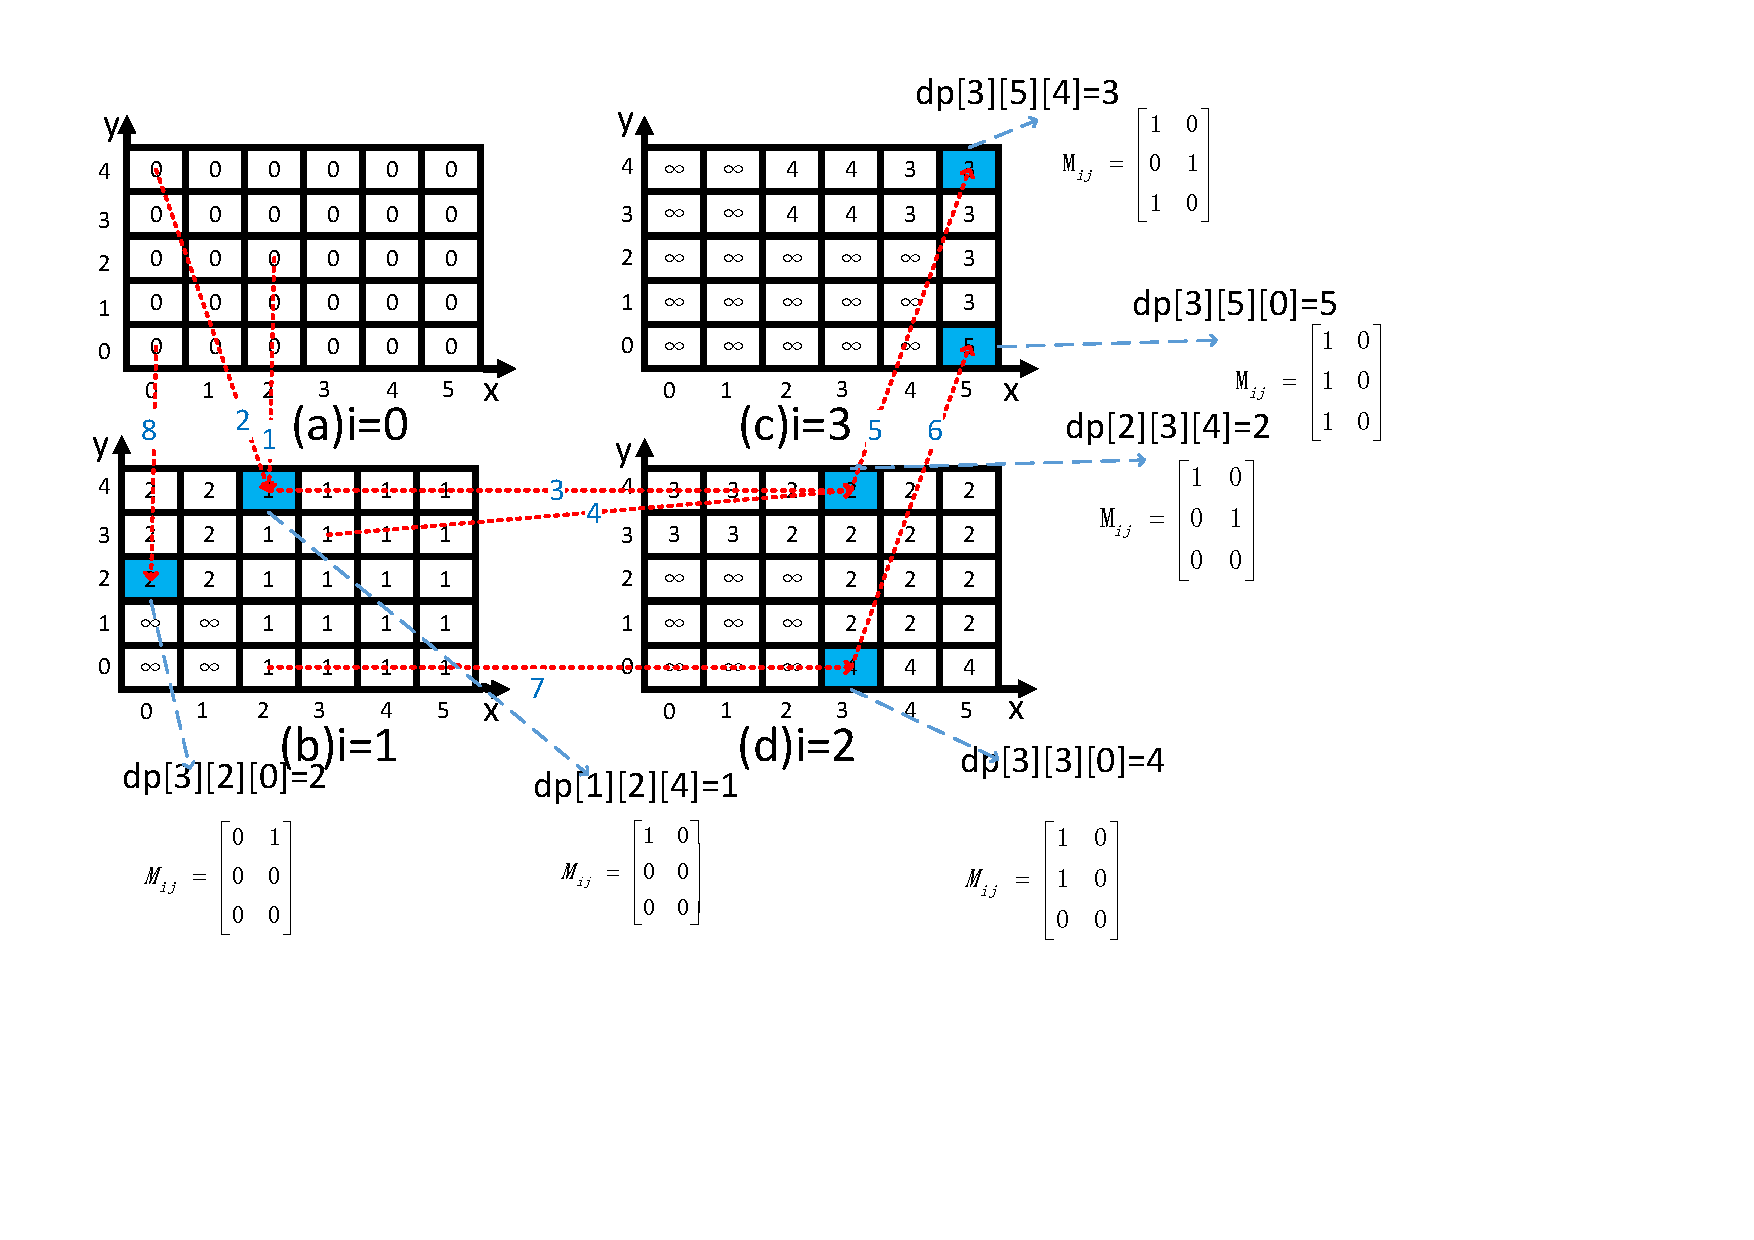
\includegraphics[width=5in]{figures/DPIllustration}\\
  \caption{Three virtual node, the first virtual node could be placed to first and second physical node,  the second virtual node could be placed to first and second physical node,  the third virtual node could only be placed to first physical node.  The  node computation capacity of first physical node is 5, the node computation capacity of second physical node is 4. $w_{ij}$=[1,2;3,1;1,$\infty$].}\label{fig:DPIllustration}
\end{figure}


\begin{algorithm}
\label{alg:DPAlg}
\caption{基于动态规划方法二分星型图匹配算法}
\begin{algorithmic}[1]
\REQUIRE {$dp[i][{x_1}][{x_2}] \ldots [{x_m}]=0(1\leq i \leq n, 0\leq x_1\leq c_1, 0\leq x_2\leq c_2,\ldots, 0\leq x_m\leq c_m)$ is firstly assigned as infinity $\infty$, $dp[0][{x_1}][{x_2}] \ldots [{x_m}]=0(0\leq x_1\leq c_1, 0\leq x_2\leq c_2,\ldots, 0\leq x_m\leq c_m)$, m is the number of physical nodes. $M[{x_1}][{x_2}] \ldots [{x_m}]=\textbf{0}_{n\times m}$ is placement of every virtual node.}
\ENSURE {obtaining optimal virtual node's placement when node up-bound capacity of physical nodes is $c_1,c_2,\ldots,c_m$, respectively.}
\FORALL{$i$ such that $1\leq i\leq n$ }
\FORALL{$x_1,x_2,\ldots,x_m$ such that $ c_1\geq x_1\geq d_i$, $c_2\geq x_2\geq d_i$,$c_3\geq x_3\geq d_i$,$c_m\geq x_m\geq d_i$}

\STATE {$dp[i][{x_1}][{x_2}] \ldots [{x_m}] = min\{\theta (i,1),\theta (i,2),\ldots,\theta (i,j),\ldots,\theta (i,m)\}$}

\STATE{$j' = \mathop {\arg \min }\limits_j \{\theta (i,1),\theta (i,2),\ldots,\theta (i,j),\ldots,\theta (i,m)\}$, }.
\STATE{$M[{x_1}][{x_2}] \ldots [{x_m}]=M[{x_1}][{x_2}] \ldots[x_{j'}-d_i]\ldots [{x_m}]$}
\STATE{$M[{x_1}][{x_2}] \ldots [{x_m}]_{ij'}=1$}
\ENDFOR
\ENDFOR
\RETURN $dp[i][{c_1}][{c_2}] \ldots [{c_m}]$ and $M[{c_1}][{c_2}] \ldots [{c_m}]$
\end{algorithmic}
\end{algorithm}

为了清晰地表示,在本例中,需要将三个虚拟星型图放置到两个可用的物理星型图以实现最小的备份资源成本。物理节点下的可用容量分别为$c_1=5$ 和$c_2=4$。 这三颗虚拟星型图的容量需求分别为$d_1=2$,$d_2=1$和 $d_3=2$。在这些虚拟星型图中需要执行的虚拟功能是$f(1)=f_1$, $f(2)=f_1$, $f(3)=f_2$。这两个物理节点支持的虚拟功能是$F(1)=\{f_1,f_2\}$ 和$F(2)=\{f_1\}$。

在图\ref{fig:DPIllustration}中, $x$和 $y$轴分别表示物理星型图$s_1$ 和$s_2$ 的容量极限。虚拟星型图与物理星型图的连接边的权重$w_{11}=1$, $w_{12}=2$, $w_{21}=3$, $w_{22}=1$, $w_{31}=1$, $w_{32}=\infty$。 最初,在图\ref{fig:DPIllustration}(a) 中,由于没有对任何物理星型图放置虚拟星型图,所有容量限制情况下的备份成本($x_1$=0,1,2,3,4和$x_2$=0,1,2,3,4,5) 都是0。特别是,即使设置了4 和5 的容量限制,dp[0][4][5]=0。在图\ref{fig:DPIllustration}(b) 中,当将容量要求为$d_1=1$ 的第一个虚拟节点$v_1$ 放置到这两个物理节点时,可以在两个物理节点中执行$f_1$。因此,我们有
\begin{equation}
dp[1][{x_1}][{x_2}] = \min \{\theta (1,1),\theta (1,2)\}
\end{equation}

特别是,如果这两个物理节点的容量极限分别为$x_1$=2和$x_2$=0,则$dp[1][2][0]= dp[0][0][0]+w_{11}=2$。如果这两个物理节点的容量极限分别为$x_1$=2和$x_2$=4,则$\theta (1,1)=dp[0][0][2]+w_{11}$和$\theta (1,2)=\infty$,从而$dp[1][2][4]=min\{ dp[0][0][4]+w_{11}), dp[0][2][2]+w_{12} \}=1$。

同样,当将容量要求$d_2=2$的第二个虚拟节点放置到这两个物理节点时,所有容量限制下的成本结果如图\ref{fig:DPIllustration}(d)所示。因为$f_2$ 可以在两个物理节点中执行,因此$v_2$可以放置在两个物理节点中,所以我们有
\begin{equation}
dp[2][{x_1}][{x_2}] = \min \{\theta (2,1),\theta (2,2)\}
\end{equation}


特别是,如果这两个物理节点的容量极限分别为$x_1$=3和$x_2$=4,则$dp[2][3][4]=min\{dp[1][2][4]+w(2,1)$,$dp[1][3][3]+w(2,2)\}=2$。如果这两个物理节点的容量极限分别为$x_1$=3和$x_2$=0,则$dp[2][3][0]=dp[1][2][0]+w(2,1)=4$。图\ref{fig:DPIllustration}(d) 显示了将容量要求为$d_3=1$的第三个虚拟节点放置到这两个物理节点时的最小资源成本结果。由于$f_3$只能在物理节点$s_1$中执行,所以我们有$\theta (3,2)=\infty$。 特别是,如果这两个物理节点的容量极限分别为$x_1$=5 和$x_2$=0,则$dp[3][5][0]=dp[2][3][0]+w(3,1)=4$。由于这两个物理节点的节点能力分别为5 和4,我们得到了$dp[3][5][4]=dp[2][3][4]+w(3,1)=3$,如图\ref{fig:DPIllustration}(d)所示,在dp[3][5][4]=3处得到了最佳位置,赋值为$v_1\rightarrow s_1, v_2\rightarrow s_2, v_3\rightarrow s_1$。

例如,如图\ref{fig:StarRepresentation}和等式\ref{lab:Node1FaliureAlignmentMatrixNew} 所示,最优M赋值如下:
\begin{equation}
M_{ij}=\left[ {\begin{array}{*{20}{c}}
0&0&0&0&1&0&0\\
1&0&0&0&0&0&0\\
0&1&0&0&0&0&0\\
0&0&1&0&0&0&0
\end{array}} \right]
\end{equation}
\section{巧妙避免添加备份资源}
如果一个节点失败,则在应用算法\ref{alg:DPAlg}计算最小额外资源后,添加新的物理节点和物理路径来维护网络服务。如果不包含任何虚拟节点的物理节点在节点失效前就添加为备份节点,我们应该将这个物理节点设置为a=1,以指示该物理节点已经容纳虚拟节点。

由于我们的可生存虚拟网络嵌入问题是为了最小化在任何一个节点失效时所增加的备份资源,而不是给定的一个节点故障,我们应该逐一测试每个节点的故障,并添加足够的备份资源。作为备份资源只需要当节点失效时,备份资源应在不同节点失效时共享。如果我们直接应用(\ref{eq:edge weight}) 中定义的成本来计算另一个物理节点失效时的备份资源,因为(\ref{eq:edge weight}) 中定义的成本不考虑备份资源共享,则会导致重复添加备份资源的问题。

为了解决这一问题,我们将$M(j)$加入到物理星型结构中,表示在节点失效的情况下迁移到物理节点$s_j$中的虚拟节点集。
\begin{equation}
PhysicalStar(s_j)=(s_j, \phi^{-1}( s_j), c_j, F(j), \phi(N(\phi^{-1}( s_j))), a, M(j))
\end{equation}
由于备份资源应该只添加一次,为了便于表示该约束,我们定义了以下约束。
\begin{equation}
\mu (x) = \left\{ {\begin{array}{*{20}{c}}
   x & {x > 0}  \\
   0 & {x \le 0}  \\
\end{array}} \right.
\end{equation}
当我们测试另一个节点失效时,而不是等式\ref{eq:edge weight}中定义的代价,我们定义了一个新的代价函数,考虑到不同节点失败时的备份资源共享。

如等式\ref{eq:new edge weight}所示,资源成本是根据两种情况设置的。如果虚拟节点$v_i$ 最初由物理服务器$s_j$持有,或者$v_i$被迁移到物理服务器,即${{v_i} \in \left( {{\phi ^{ - 1}}({s_j}) \cup M(j)} \right)}$,当它的邻居$v_k \in N(i)$(${\phi \left( k \right) \notin \phi \left( {{\phi ^{ - 1}}({s_j})} \right)}$)失效时,路径带宽成本为${\sum\limits_{k \in N(i) \cap N(i')} {\mu({d_{ik}} - {d_{i'k}})}  + \sum\limits_{k \in \left( {N(i) - N(i')} \right)} {{d_{ik}}} }$。

\begin{figure*}
  \centering
  % Requires \usepackage{graphicx}
    \begin{equation}
  \footnotesize
w(i,j) = \left\{ {\begin{array}{*{20}{c}}
   {\sum\limits_{k \in N(i) \cap N(i')} {\mu({d_{ik}} - {d_{i'k}})}  + \sum\limits_{k \in \left( {N(i) - N(i')} \right)} {{d_{ik}}} } & {{v_i} \in \left( {{\phi ^{ - 1}}({s_j}) \cup M(j)} \right),{v_{i'}} \in M(j),k \notin \phi \left( {{\phi ^{ - 1}}({s_j})} \right)}  \\
   {\sum\limits_{k \in N(i) \cap N(i')} {\mu({d_{ik}} - {d_{i'k}})}  + \sum\limits_{k \in \left( {N(i) - N(i')} \right)} {{d_{ik}}}  + \lambda f({d_i} - \mathop {\max }\limits_{{v_{i'}}} \left( {{d_{i'}}} \right)) + \beta {M_m} + \theta } & {{v_i} \notin \left( {{\phi ^{ - 1}}({s_j}) \cup M(j)} \right),{v_{i'}} \in M(j)}  \\
\end{array}} \right.
    \label{eq:new edge weight}
    \end{equation}
\end{figure*}

否则,在原先节点失效的测试前这个虚拟节点$v_i$没有被一个物理节点持有和迁移到其他物理节点,除了这个带宽成本为${\sum\limits_{k \in N(i) \cap N(i')} {\mu({d_{ik}} - {d_{i'k}})}  + \sum\limits_{k \in \left( {N(i) - N(i')} \right)} {{d_{ik}}} }$,节点的容量成本为${\lambda * \mu({d_i} - \mathop {\max }\limits_{{v_{i'}}} \left( {{d_{i'}}} \right))}$,虚拟服务器迁移的代价为${\beta * {M_m}}$ 和 $\theta$从映射虚拟星型图$v_i$到物理星型图$s_j$。如${\mu({d_i} - \mathop {\max }\limits_{{v_{i'}}} \left( {{d_{i'}}} \right))}$ 而言,如果备份容量已分配的最大值${\mathop {\max }\limits_{{v_{i'}}} \left( {{d_{i'}}} \right)}$大于当前映射(即$d_i$),不需要任何资源,否则,备份资源还缺少${{d_i} - \mathop {\max }\limits_{{v_{i'}}} \left( {{d_{i'}}} \right)}$。

对于$VirtualStar(v_2)$,由于$v_3$最初由$s_3$持有,但是当物理节点$s_1$ 失效时,我们可以将虚拟节点$v_3$迁移到物理节点$s_2$,因为$s_2$ 是以前已经安装过虚拟机,因此,成本包括虚拟链路带宽成本$11$,节点容量成本5,虚拟机迁移成本$M_m$。

基于节\ref{lab:DynamicProgrammingEquation}的方法,在物理节点$s_1$失效时得到最佳节点映射:$v_1 \rightarrow s_5$, $v_2 \rightarrow s_2$, $v_3 \rightarrow s_3$, $v_4 \rightarrow s_4$。物理节点$s_5$ 开始为虚拟节点$v_1$建立和应用2个节点计算资源,并分别找到带宽约束为4、5、3 的对应的虚拟链路$(v_1,v_2),(v_1,v_3),(v_1,v_4)$的三个物理路径。

如图\ref{fig:StarRepresentationNode2}所示展示了二分图的一个例子,物理节点$s_2$ 在物理节点$s_1$失效之后再失效。这个二分图的边权矩阵可以用矩阵\ref{lab:Node2FaliureAlignmentMatrixNew}表示。
\begin{equation*}
\small{
 {\begin{array}{*{20}{c}}
&R_{S_{1}}&R_{S_{2}}&R_{S_3}&R_{S_4}&R_{S_5}&R_{S_6}&R_{S_{7}}\\
{L_{V_1}}&\fbox{4}&\infty&\infty&\infty&M_{m}&C_{s}+M_{m}+(2)+12&\infty\\
L_{V_2}&\infty&\infty&\infty&\infty&\fbox{$M_{m}$+(1)+5}&\infty&C_{s}+M_{m}+(3)+10\\
L_{V_3}&\infty&\infty&\fbox{5}&\infty&\infty&\infty&C_{s}+M_{m}+(5)+11\\
L_{V_4}&\infty&\infty&\infty&\fbox{3}&\infty&C_{s}+M_{m}+(6)+3&\infty\\
\end{array}}
}
\label{lab:Node2FaliureAlignmentMatrixNew}
\end{equation*}

\begin{figure}
\centering
% Requires \usepackage{graphicx}
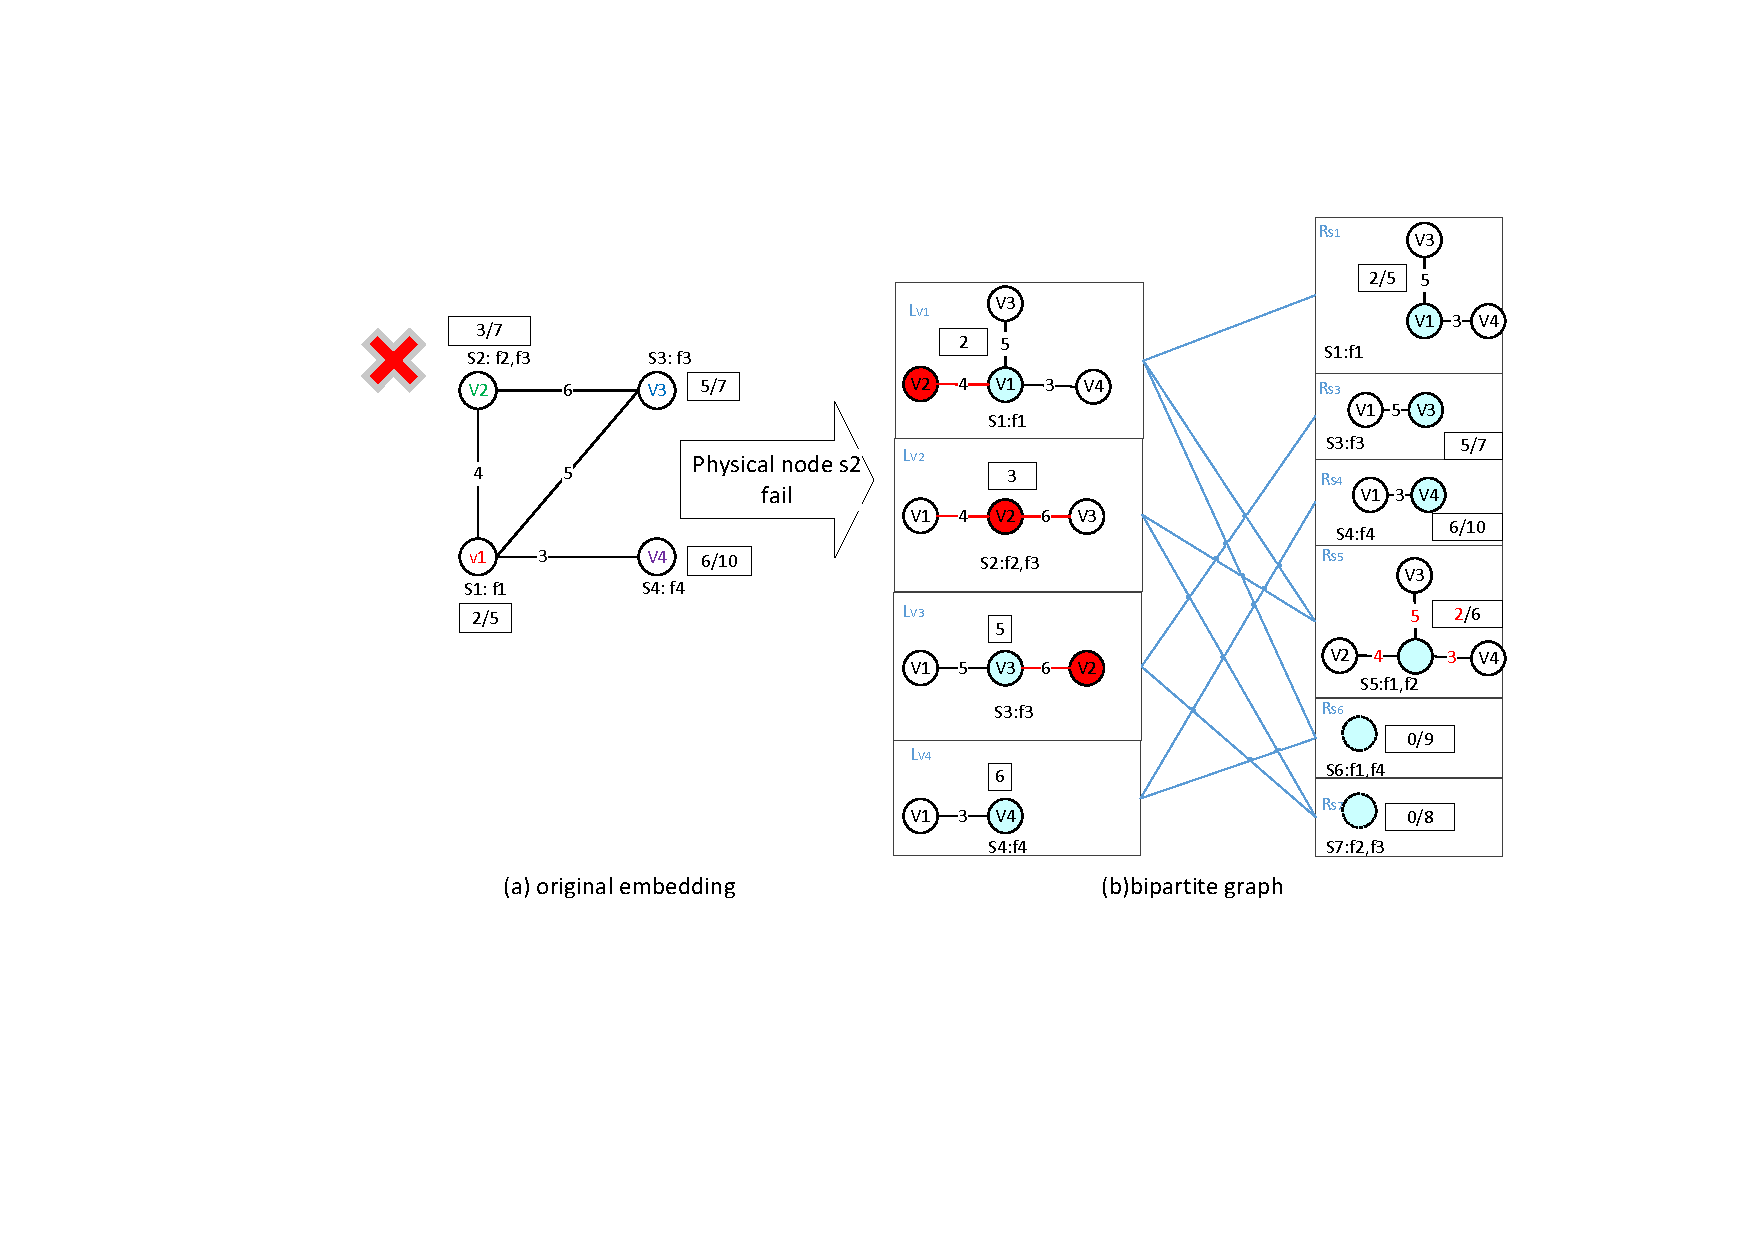
\includegraphics[width=4in]{figures/StarRepresentationNode2}\\
  \caption{Components of VirtualStar($v_i$) and PhysicalStar($s_j$) when physical node $s_2$ fail}\label{fig:StarRepresentationNode2}
\end{figure}
\section{实验环境与评价指标}
对于任何VN请求,VN节点的数目是由3到10之间的均匀分布随机确定的,每一对虚拟节点都是随机的与概率0.5有关。VN节点的计算需求从1到5之间分布一致,并且VN上的带宽从1到10。

VN请求的到达采用泊松过程建模(平均每1时间单位请求15次)。请求的持续时间服从指数分布,平均有100个时间单位,高的请求率和较长的租用时间保证了物理基础设施的高利用率。

根据\cite{armbrust2009above,yu2010survivable},即$\lambda/\alpha=\RelativeCostbetweenComputingBandwidth$,节点的计算资源与链路的带宽资源的相对成本为3。使用的SN 拓扑是SNDlib拓扑数据\cite{orlowski2010sndlib}。底层物理节点(链路)的计算(带宽)资源是整数的。分别分布在10~20(50 和100)之间。为了对设备节点失效场景进行建模,我们选择了底层物理网络中的所有底层物理设备节点逐个失效,并统计计算了每24 个时间单元的迁移频率。


\section{算法性能评估及比较}
\section{本章小节}
